\documentclass{article}
\usepackage[paperwidth=14.0cm,paperheight=8.0cm,margin=0.2cm]{geometry}
\usepackage{amsmath,amssymb}
\usepackage{xcolor}
\usepackage{tikz}
\usetikzlibrary{arrows.meta,positioning,calc,fit,shapes.geometric,backgrounds}

\begin{document}
\pagestyle{empty}
\centering

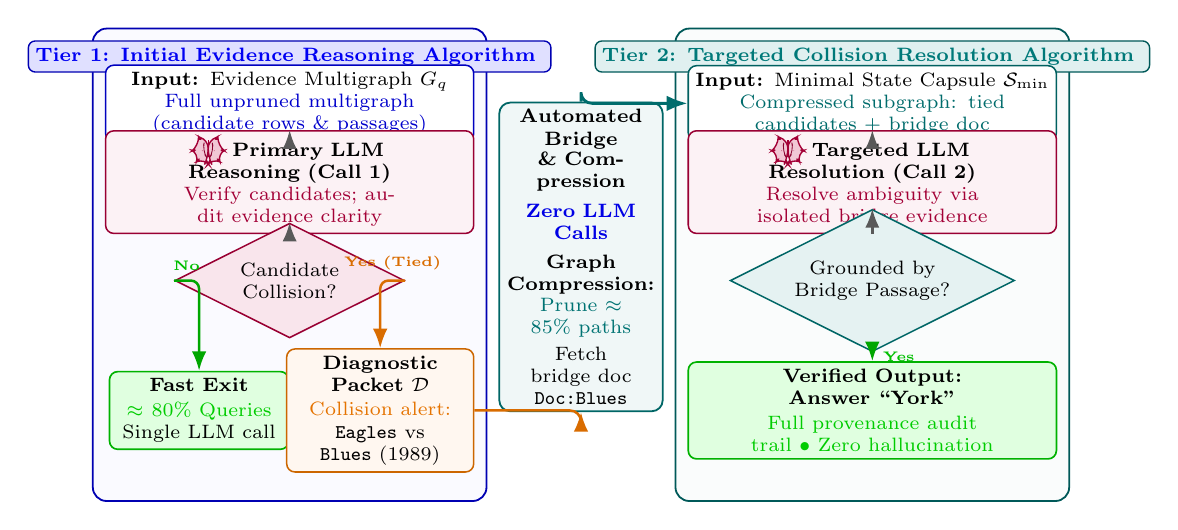
\begin{tikzpicture}[
  >=Latex,
  font=\sffamily\scriptsize,
  % Panels
  col_panel/.style={draw=#1!70!black, fill=#1!2!white, rounded corners=5pt, line width=0.65pt},
  col_hdr/.style={fill=#1!12, draw=#1!70!black, line width=0.5pt, rounded corners=2.5pt, font=\bfseries\scriptsize, text=#1!95!black, inner sep=2.5pt, align=center},
  % Flowchart Nodes
  fc_box/.style={draw=#1!75!black, fill=white, rounded corners=3pt, line width=0.55pt, inner sep=2.5pt, align=center, font=\scriptsize},
  fc_proc/.style={draw=purple!80!black, fill=purple!5, rounded corners=3pt, line width=0.55pt, inner sep=2.5pt, align=center, font=\scriptsize},
  fc_dec/.style={diamond, aspect=2.0, draw=#1!80!black, fill=#1!10, line width=0.55pt, inner sep=1.0pt, align=center, font=\scriptsize},
  fc_exit/.style={draw=green!70!black, fill=green!12, rounded corners=3pt, line width=0.6pt, inner sep=2.5pt, align=center, font=\scriptsize},
  fc_out/.style={draw=orange!80!black, fill=orange!6, rounded corners=3pt, line width=0.55pt, inner sep=2.5pt, align=center, font=\scriptsize},
  % Bridge Box
  bridge_box/.style={draw=teal!80!black, fill=teal!6, rounded corners=4pt, line width=0.65pt, inner sep=2.5pt, align=center, font=\scriptsize},
  % Arrows
  arr/.style={->, line width=0.85pt, draw=gray!70!black},
  arr_green/.style={->, line width=0.9pt, draw=green!65!black},
  arr_orange/.style={->, line width=0.9pt, draw=orange!85!black},
  arr_bridge/.style={->, line width=1.0pt, draw=teal!85!black}
]

% Brain icon pic
\tikzset{
  brain_icon/.pic={
    \begin{scope}[scale=0.17]
      \draw[fill=purple!22, draw=purple!85!black, line width=0.5pt]
        (0, 0.72) 
        .. controls (-0.35, 0.82) and (-0.72, 0.62) .. (-0.72, 0.28)
        .. controls (-0.92, 0.12) and (-0.92, -0.22) .. (-0.68, -0.34)
        .. controls (-0.76, -0.58) and (-0.52, -0.78) .. (-0.28, -0.68)
        .. controls (-0.18, -0.82) and (-0.05, -0.68) .. (0, -0.58)
        -- cycle;
      \draw[fill=purple!22, draw=purple!85!black, line width=0.5pt]
        (0, 0.72) 
        .. controls (0.35, 0.82) and (0.72, 0.62) .. (0.72, 0.28)
        .. controls (0.92, 0.12) and (0.92, -0.22) .. (0.68, -0.34)
        .. controls (0.76, -0.58) and (0.52, -0.78) .. (0.28, -0.68)
        .. controls (0.18, -0.82) and (0.05, -0.68) .. (0, -0.58)
        -- cycle;
      \draw[purple!85!black, line width=0.5pt] (0, 0.70) -- (0, -0.56);
      \fill[purple!85!black] (-0.35, 0.3) circle (0.75pt);
      \fill[purple!85!black] (-0.45, -0.1) circle (0.75pt);
      \fill[purple!85!black] (-0.25, -0.4) circle (0.75pt);
      \draw[purple!70!black, line width=0.3pt] (-0.35, 0.3) -- (-0.45, -0.1) -- (-0.25, -0.4);
      \fill[purple!85!black] (0.35, 0.3) circle (0.75pt);
      \fill[purple!85!black] (0.45, -0.1) circle (0.75pt);
      \fill[purple!85!black] (0.25, -0.4) circle (0.75pt);
      \draw[purple!70!black, line width=0.3pt] (0.35, 0.3) -- (0.45, -0.1) -- (0.25, -0.4);
    \end{scope}
  }
}

% -------------------------
% COLUMN 1: TIER 1 ALGORITHM
% Center X = 2.6cm, Width = 5.0cm (X: 0.1 to 5.1)
% -------------------------
\node[col_panel=blue, minimum width=5.0cm, minimum height=6.0cm] (c1) at (2.6, 0) {};
\node[col_hdr=blue, minimum width=4.7cm, anchor=north] (t1_hdr) at ([yshift=-1.6mm]c1.north) {
  Tier 1: Initial Evidence Reasoning Algorithm
};

% T1 Step 1: Input Box
\node[fc_box=blue, text width=4.5cm] (t1_in) at (2.6, 2.05) {
  \textbf{Input:} Evidence Multigraph $G_q$\\
  \textcolor{blue!80!black}{Full unpruned multigraph (candidate rows \& passages)}
};

% T1 Step 2: Primary LLM Reasoning
\node[fc_proc, text width=4.5cm] (t1_proc) at (2.6, 1.05) {
  \tikz[baseline=-2.5pt]{\pic {brain_icon};}\hspace{4pt}\textbf{Primary LLM Reasoning (Call 1)}\\
  \textcolor{purple!85!black}{Verify candidates; audit evidence clarity}
};

% T1 Step 3: Decision Diamond (Centered at 2.6)
\node[fc_dec=purple, text width=1.8cm] (t1_dec) at (2.6, -0.2) {
  Candidate\\Collision?
};

% T1 Step 4a: Fast Exit (Branch: No collision, left bottom)
\node[fc_exit, text width=2.1cm] (t1_exit) at (1.45, -1.85) {
  \textbf{Fast Exit}\\[0.3mm]
  \textcolor{green!80!black}{$\approx 80\%$ Queries}\\
  Single LLM call
};

% T1 Step 4b: Diagnostic Packet (Branch: Collision detected, right bottom)
\node[fc_out, text width=2.2cm] (t1_out) at (3.75, -1.85) {
  \textbf{Diagnostic Packet $\mathcal{D}$}\\[0.3mm]
  \textcolor{orange!90!black}{Collision alert:}\\
  \texttt{Eagles} vs \texttt{Blues} (1989)
};

% Connectors in Tier 1
\draw[arr] (t1_in) -- (t1_proc);
\draw[arr] (t1_proc) -- (t1_dec);
\draw[arr_green, rounded corners=3pt] (t1_dec.west) -| node[above, font=\bfseries\tiny, text=green!75!black, near start] {No} (t1_exit.north);
\draw[arr_orange, rounded corners=3pt] (t1_dec.east) -| node[above, font=\bfseries\tiny, text=orange!85!black, near start] {Yes (Tied)} (t1_out.north);


% -------------------------
% COLUMN 2: TIER 2 ALGORITHM
% Center X = 10.0cm, Width = 5.0cm (X: 7.5 to 12.5)
% -------------------------
\node[col_panel=teal, minimum width=5.0cm, minimum height=6.0cm] (c2) at (10.0, 0) {};
\node[col_hdr=teal, minimum width=4.7cm, anchor=north] (t2_hdr) at ([yshift=-1.6mm]c2.north) {
  Tier 2: Targeted Collision Resolution Algorithm
};

% T2 Step 1: Input Box
\node[fc_box=teal, text width=4.5cm] (t2_in) at (10.0, 2.05) {
  \textbf{Input:} Minimal State Capsule $\mathcal{S}_{\mathrm{min}}$\\
  \textcolor{teal!85!black}{Compressed subgraph: tied candidates + bridge doc}
};

% T2 Step 2: Targeted LLM Call
\node[fc_proc, text width=4.5cm] (t2_proc) at (10.0, 1.05) {
  \tikz[baseline=-2.5pt]{\pic {brain_icon};}\hspace{4pt}\textbf{Targeted LLM Resolution (Call 2)}\\
  \textcolor{purple!85!black}{Resolve ambiguity via isolated bridge evidence}
};

% T2 Step 3: Decision Diamond
\node[fc_dec=teal, text width=2.4cm] (t2_dec) at (10.0, -0.2) {
  Grounded by\\Bridge Passage?
};

% T2 Step 4: Final Verified Answer
\node[fc_exit, text width=4.5cm] (t2_out) at (10.0, -1.85) {
  \textbf{Verified Output: Answer ``York''}\\[0.4mm]
  \textcolor{green!80!black}{Full provenance audit trail $\bullet$ Zero hallucination}
};

% Connectors in Tier 2
\draw[arr] (t2_in) -- (t2_proc);
\draw[arr] (t2_proc) -- (t2_dec);
\draw[arr_green] (t2_dec.south) -- node[right, font=\bfseries\tiny, text=green!75!black] {Yes} (t2_out.north);


% -------------------------------------------------------------
% CENTER CONNECTOR: BRIDGE SEARCH & GRAPH COMPRESSION
% Center X = 6.3cm, Width = 2.0cm (X: 5.3 to 7.3)
% -------------------------------------------------------------
\node[bridge_box, text width=1.9cm] (bridge) at (6.3, 0.1) {
  \textbf{Automated Bridge}\\[-0.2mm]
  \textbf{\& Compression}\\[1.0mm]
  \textcolor{blue!90!black}{\textbf{Zero LLM Calls}}\\[0.8mm]
  \textbf{Graph Compression:}\\[-0.2mm]
  \textcolor{teal!90!black}{Prune $\approx 85\%$ paths}\\[0.6mm]
  Fetch bridge doc\\
  \texttt{Doc:Blues}
};

% Inter-tier connecting flow
\draw[arr_orange, rounded corners=4pt] (t1_out.east) -- (6.3, -1.85) -- (bridge.south);
\draw[arr_bridge, rounded corners=4pt] (bridge.north) -- (6.3, 2.05) -- (t2_in.west);

\end{tikzpicture}
\end{document}
